\documentclass{article}
\usepackage[utf8]{inputenc}
% important for graphicx
\usepackage{graphicx}
\graphicspath{ {img/} }
\usepackage{float}
\usepackage{hyperref}
\usepackage{enumitem}
\usepackage[]{algorithm2e}
% background color for definitions
\usepackage[most]{tcolorbox}
\tcbset{
    frame code={}
    center title,
    left=0pt,
    right=0pt,
    top=0pt,
    bottom=0pt,
    colback=blue!6!white,
    colframe=white,
    width=\dimexpr\textwidth\relax,
    enlarge left by=0mm,
    boxsep=10pt,
    arc=0pt,outer arc=0pt,
}


\begin{document}

\title{Image Processing II\\
 Watershed}
\author{Aadil Anil Kumar \\
Otmane Sabir
}
\date{29/2/2020}
\maketitle
\vspace{10mm}
\begin{center}
\section*{Introduction}
\large
The second homework assignment required us to implement the watershed transform while following certain guidelines which could be summarized to the following list: 
\vspace{7mm}
\begin{enumerate}
    \item Implement the watershed algorithm as described as pseudo code from the \hyperref[sec:hello]{\textcolor{blue}{textbook}} 4-connected and 8-connected neighborhood.
    \item Output a single CSV file for the transformed image in the same format and same definition and value domains as the input image 'f'.
    \item Do meaningful (motivated from a real-world perspective) watersheds for 3 other images.
\end{enumerate}
\end{center}
\newpage

\tableofcontents

\newpage

\section{Watershed Transform}
\vspace{2mm}
\begin{flushleft}
The watershed transform is a classical segmentation - separating different objects in an image - algorithm in the world of image processing; it initially derives from the the geological watershed which means the elevated terrain that separates neighboring drainage basins. The watershed transform segmentation follows the same logic: starting from defined markers, the watershed algorithm treats pixels values as a local topography (elevation). The algorithm floods basins from the markers until basins attributed to different markers meet on watershed lines. \textif{See Figure \ref{fig:watershed_visualization}}\newline
\vspace{2mm}
\end{flushleft}
\begin{figure}[ht]
    \centering
    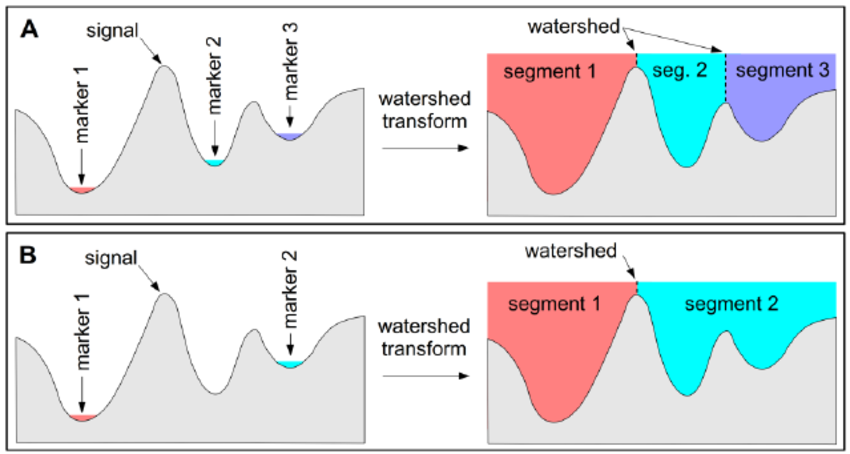
\includegraphics[width=8cm]{watershed.png}
    \caption{Watershed Visualization}
    \label{fig:watershed_visualization}
\end{figure}
\subsection{Formal Definition:}
\begin{flushleft}
\vspace{2mm }
\begin{tcolorbox}
\textsc{Definition: }\cite{parwshed} \newline\newline

Let $f \in C(D)$ have $minima$ $\{m_{k}\}_{k \in I}$, for some index set $I$. The catchment basin $CB(m_i)$ of a minimum $m_i$ is defined as the set of points $x \in D$ which are topographically closer to $m_i$ than to any other regional minimum $m_j$:

\newline

\begin{center}
\begin{equation*}
    CB(m_i) = \{x \in D | \forall j \textbackslash \in I\{i\} : f(m_i) + T_f(x, m_i) < f(m_j) + T_f(x, m_j)\}
\end{equation*}
\end{center}
\vspace{2mm}
The watershed of $f$ is the set of points which do not belong to any catchment
\begin{center}
\begin{equation*}
Wshed(f) = D \cap \left(\bigcup\limits_{i \in I} CB(m_i)\right)^c.
\end{equation*}
\end{center}
\vspace{4mm}
Let $W$ be some label, $W \notin I$. The watershed transform of $f$ is a mapping $\lambda : D \to I \cup \{W\}$, such that $\lambda(p) = i$ if $p \in CB(m_i)$, and $\lambda(p) = W$ if $p \in Wshed(f)$.
\newline\newline\newline
So the watershed transform of $f$ assigns labels to the points of $D$, such that $(i)$ different catchment basins are uniquely labelled, and $(ii)$ a special label $W$ is assigned to all points of the watershed of $f$.
\end{tcolorbox}
\end{flushleft}



\section{Algorithmic Definition}
\vspace{2mm}
In our implementation, we're relying on the simulated immersion approach introduced by Vincent \& Soille \cite{soilletextbook}. \newline\newline
Metaphorically speaking, the algorithm pierces holes in every minimum, and the entire relief begins to be flooded with water. Starting from the minimum of lowest height, the water gradually fills up all catchment basins. Watersheds are built in the places where water from different basins unites. The process ends when the water reaches the maximum peak of the relief, and as a result, every catchment basin gets covered by the watershed lines which are easily distinguishable lines from the rest of the output.
\subsection{Formal Definition}
\subsection{Implementation}
\subsubsection{Pixel Mapping}
\subsubsection{Neighbouring Pixels}
\subsubsection{Queue Data Structure}

\section{Experiments & Results}


\section{Comparison}


\section{Task Distribution}


\newpage

\begin{thebibliography}{9}
\label{sec:hello}



\bibitem{parwshed}
Jos B.T.M. Roerdink and Arnold Meijster : \newline
Institute for Mathematics and Computing Science, 
\\\texttt{http://www.cs.rug.nl/roe/publications/parwshed.pdf}


\bibitem{soilletextbook} 
Soille, P. (2010). Morphological image analysis: principles and applications. 
\textif{Berlin: Springer. Samarin}. 

\end{thebibliography}

\end{document}
